%!TEX program = xelatex

\documentclass[compress]{beamer}
%--------------------------------------------------------------------------
% Common packages
%--------------------------------------------------------------------------
\usepackage[english]{babel}
\usepackage{pgfpages} % required for notes on second screen
\usepackage{graphicx}
\usepackage{subfigure}
\usepackage{multicol}

\usepackage{tabularx,ragged2e}
\usepackage{booktabs}

\usepackage{setspace}

%--------------------------------------------------------------------------
% Load theme
%--------------------------------------------------------------------------
\usetheme{hri}

\usepackage{dtklogos} % must be loaded after theme
\usepackage{tikz}
\usetikzlibrary{calc,mindmap,backgrounds,positioning,svg.path}

\graphicspath{{figs/}}

%--------------------------------------------------------------------------
% General presentation settings
%--------------------------------------------------------------------------
\title{Mutual Modelling in Robotics}
\subtitle{Inspiration for the Next Steps}
\date{Human-Robot Interaction, 2015, Portland}
\author{\scriptsize {\Medium Séverin Lemaignan}, Pierre Dillenbourg}
\institute{Computer-Human Interaction\\for Learning and Instruction {\Medium
EPFL}}

%--------------------------------------------------------------------------
% Notes settings
%--------------------------------------------------------------------------
%\setbeameroption{show notes on second screen}
%\setbeameroption{hide notes}

\newsavebox{\ontoinstance}
\savebox{\ontoinstance}{
\begin{tikzpicture}[
    >=latex,
    every edge/.style={<-, draw, very thick},
    every node/.style={draw, font=\sf, node distance=0.5, rounded corners,
    align=center, inner sep=5pt,fill=hriSec2Dark!50},
    classof/.style={<-, draw=black!60, dashed},
    property/.style={<-, draw=hriSec2Comp},
    propname/.style={above, draw=none, fill=none, font=\tt, inner sep=2pt},
    instance/.style={draw=hriSec1Dark, font=\sf, node distance=0.5, rounded corners,
align=center, inner sep=5pt, fill=none}]

    \node[fill=hriSec2Comp!50] (thing) {\textbf{thing}};
    \node [fill=hriSec3CompDark!50, node distance=1.8, below left=of
    thing](sthing) {place} edge[dashed] (thing);
    \node [fill=hriSec3CompDark!50, below left=of sthing] (agent) {agent} edge (sthing);
        \node [fill=hriSec3CompDark!50, below=of sthing] (artifact) {artifact} edge (sthing);
        \node [fill=hriSec3CompDark!50, below right=of sthing] (location) {physical
        support} edge (sthing);
        \node [fill=hriSec3CompDark!50, below right=of artifact] (table) {table}
            edge (location) edge (artifact);


    \node [node distance=1, below right=of thing] (tthing) {temporal thing} edge (thing);
        \node [below right=of tthing] (evt) {event} edge[dashed] (tthing);
                    \node [below right=of evt] (act) {action} edge (evt);

  \draw[dotted, thick] (-5,-5) -- (7.5, -5);

  \node [instance, below=3 of agent] (human) {human\_1} edge[classof, bend left] (agent);
  \node [instance, above right=of human, anchor=south] (robot) {pr2\_robot} edge[classof, bend left] (agent);
  \node [instance, right=of human, anchor=north west] (book) {book\_game\_thrones}
  edge[classof] (artifact);
  \node [instance, right=2 of robot] (ikea) {ikea\_table} edge[classof, bend
  right] (table);
  \node [instance, right=2 of book] (red) {red} edge[property] node[propname] {hasColor} (book);

  \draw[dotted, thick] (-5,-8) -- (7.5, -8);

  \path (book.200) edge [property, out=-100, in=-80, looseness=2]
  node[propname,auto] {isNextTo} (human.south);
  \path (book.270) edge [property, out=-100, in=-90, looseness=3.5] node[propname,auto] {looksAt} (robot.south);
  \path (ikea.south) edge [property, out=-90, in=-80, looseness=3] node[propname, auto] {isOn} (book.320);
\end{tikzpicture}
}


\begin{document}

\imageframe{gruffalo}
\whiteimageframe{gruffalo1}
\whiteimageframe{gruffalo2}
\whiteimageframe{gruffalo3}
\whiteimageframe{gruffalo4}

\begin{frame}{Gruffalo crash course}

If $m$ stands for the mouse, $f$ for the fox, $g$ for the Gruffalo

and $p$ stands for $\exists g$

\Large

\only<1-2>{
    \begin{center}
        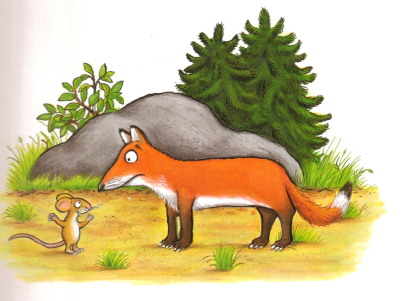
\includegraphics[width=0.3\linewidth]{gruffalo-fox}
    \end{center}

}

\only<1>{
\[
\mathsf{K}_{m}\neg p \wedge \mathsf{K}_{m}\neg\mathsf{K}_{f}\neg p 
\]
}
\only<2>{
    \begin{center}
$m$ performs action $\rightarrow \mathsf{B}_{f}p$
    \end{center}
}

\only<3>{
    \begin{center}
        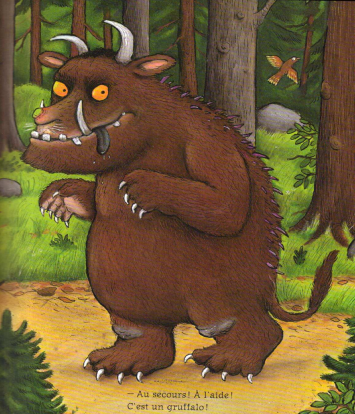
\includegraphics[width=0.3\linewidth]{gruffalo2}

$p$ stands! 
    \end{center}
}

\only<4-5>{
    \begin{center}
        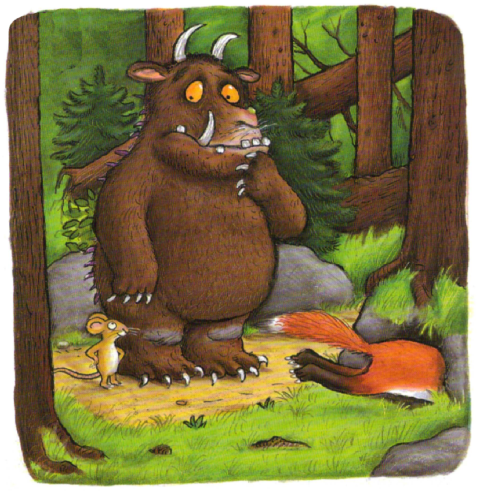
\includegraphics[width=0.3\linewidth]{gruffalo-fox2}
\[
\mathsf{B}_{g}\mathsf{K}_{f}p
\only<5>{
\wedge
\mathsf{K}_{m}\neg\mathsf{K}_{g}\mathsf{B}_{f}\neg p 
}
\]

    \end{center}


}


\end{frame}

%%%%%%%%%%%%%%%%%%%%%%%%%%%%%%%%%%%%%%%%%%%%%%%%%%%%%%%%%%%%%%%%%%%%%%%%%%%%%%%
%%%%%%%%%%%%%%%%%%%%%%%%%%%%%%%%%%%%%%%%%%%%%%%%%%%%%%%%%%%%%%%%%%%%%%%%%%%%%%%
%%%%%%%%%%%%%%%%%%%%%%%%%%%%%%%%%%%%%%%%%%%%%%%%%%%%%%%%%%%%%%%%%%%%%%%%%%%%%%%

\section{More seriously}

{
    \paper{Wimmer and Perner, {\Medium Beliefs about beliefs:
    Representation and constraining function [...]}, Cognition, 1983}
\begin{frame}{1st order ToM: the False-Belief Experiment}
    \begin{center}
    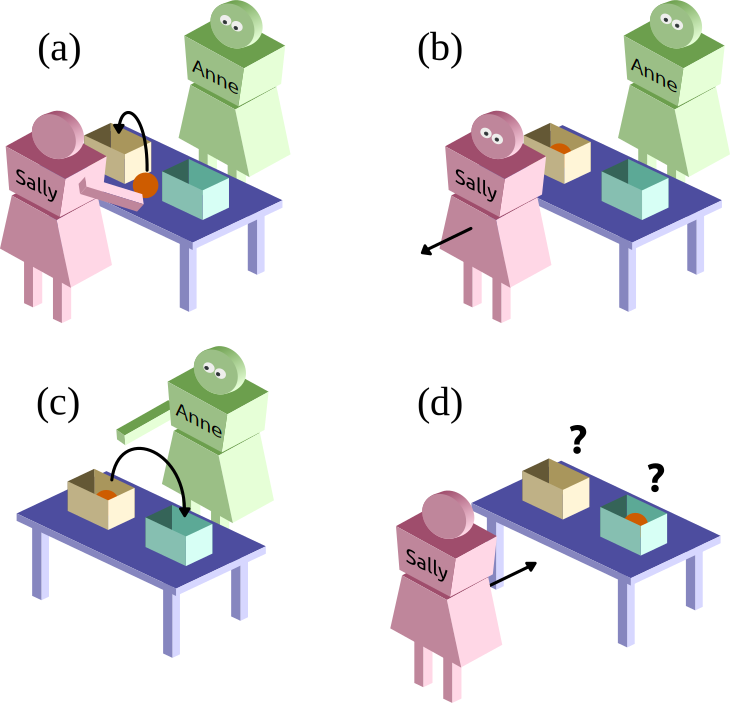
\includegraphics[width=0.7\textwidth]{sally_ann.pdf}
    \end{center}

\end{frame}
}

{ \paper{Frith and Happé, {\Medium Autism: Beyond "theory of
    mind"}, Cognition, 1994}
\begin{frame}{Deficits/Assets}
    \centering
    \begin{tabular}{p{0.5\linewidth}p{0.5\linewidth}}
        \toprule
        Elicited structed play & Spontaneous pretend play \\
        Instrumental gestures & Expressive gestures \\
        Talking about desires and emotions & Talking about beliefs and ideas \\
        Using person as tool & Using person as receiver of information \\
        Showing "active" sociability & Showing "interactive" sociability \\
        \bottomrule
    \end{tabular}
\end{frame}
}



{
    \paper{Flobbe, Verbrugge, Hendriks, Krämer,
        {\Medium Children's application of theory of mind in reasoning
    and language}, Journal of Logic, Language and
    Information, 2008}
\begin{frame}{2nd order ToM: the Chocolate Bar Experiment}
    \begin{center}
    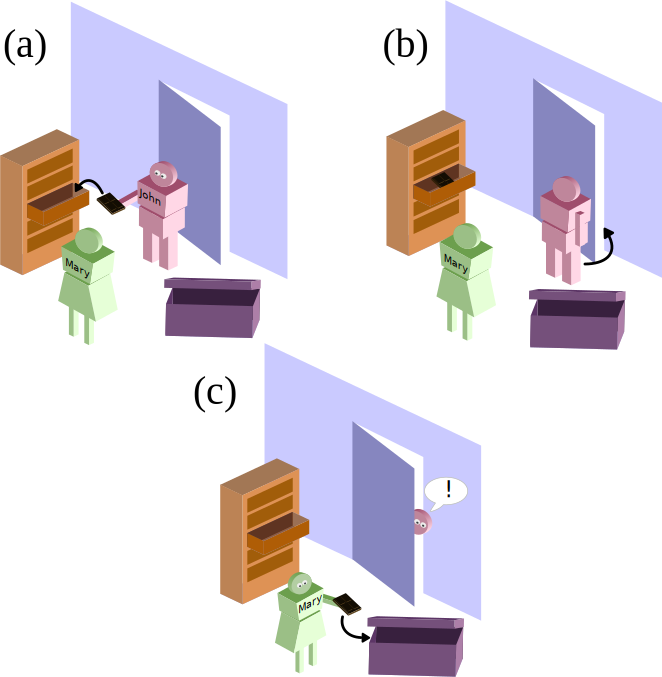
\includegraphics[width=0.7\textwidth]{chocolate-bar.pdf}
    \end{center}

\end{frame}
}

{
    \paper{Verbrugge, {\Medium Logic and social cognition}, Journal of Philosophical
    Logic, 2009}
\begin{frame}{Agreement as $\infty$-order ToM}
    \begin{center}
    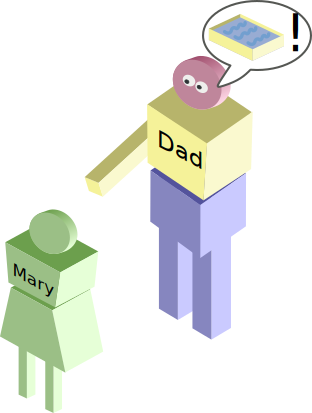
\includegraphics[width=0.2\textwidth]{mutual-agreement.pdf}
    \end{center}

    \uncover<2->{
    Shared knowledge
\[
    \mathsf{EK}_J\varphi \leftrightarrow \bigwedge_{i \in J}\mathsf{K}_i\varphi
\]
}
\uncover<3>{
    Common knowledge 
\[
    \mathsf{CK}_J\varphi \leftrightarrow
\mathsf{EK}_J\varphi \wedge \mathsf{EK}_J\mathsf{EK}_J\varphi \wedge
\mathsf{EK}_J\mathsf{EK}_J\mathsf{EK}_J\varphi \wedge ...
\]
}

\end{frame}
}



\section{Today's standards}

\begin{frame}{}
    \begin{itemize}
        \item Scassellati,
        \item Alami,
        \item Trafton with ACT-R/E
        \item Breazeal,
        \item Belpaeme,
        \item ...

    \end{itemize}
\end{frame}

{
\paper{Lemaignan, Alami, {\Medium Explicit Knowledge and the Deliberative Layer: Lessons Learned}, IROS 2013}
\begin{frame}{One Instantiation}

    \begin{center}
        \uncover<2->{
        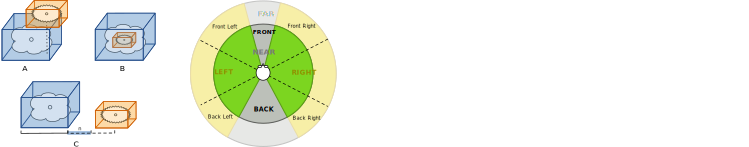
\includegraphics[width=0.9\textwidth]{spark.pdf}
    }

    \begin{multicols}{2}
        \centering
        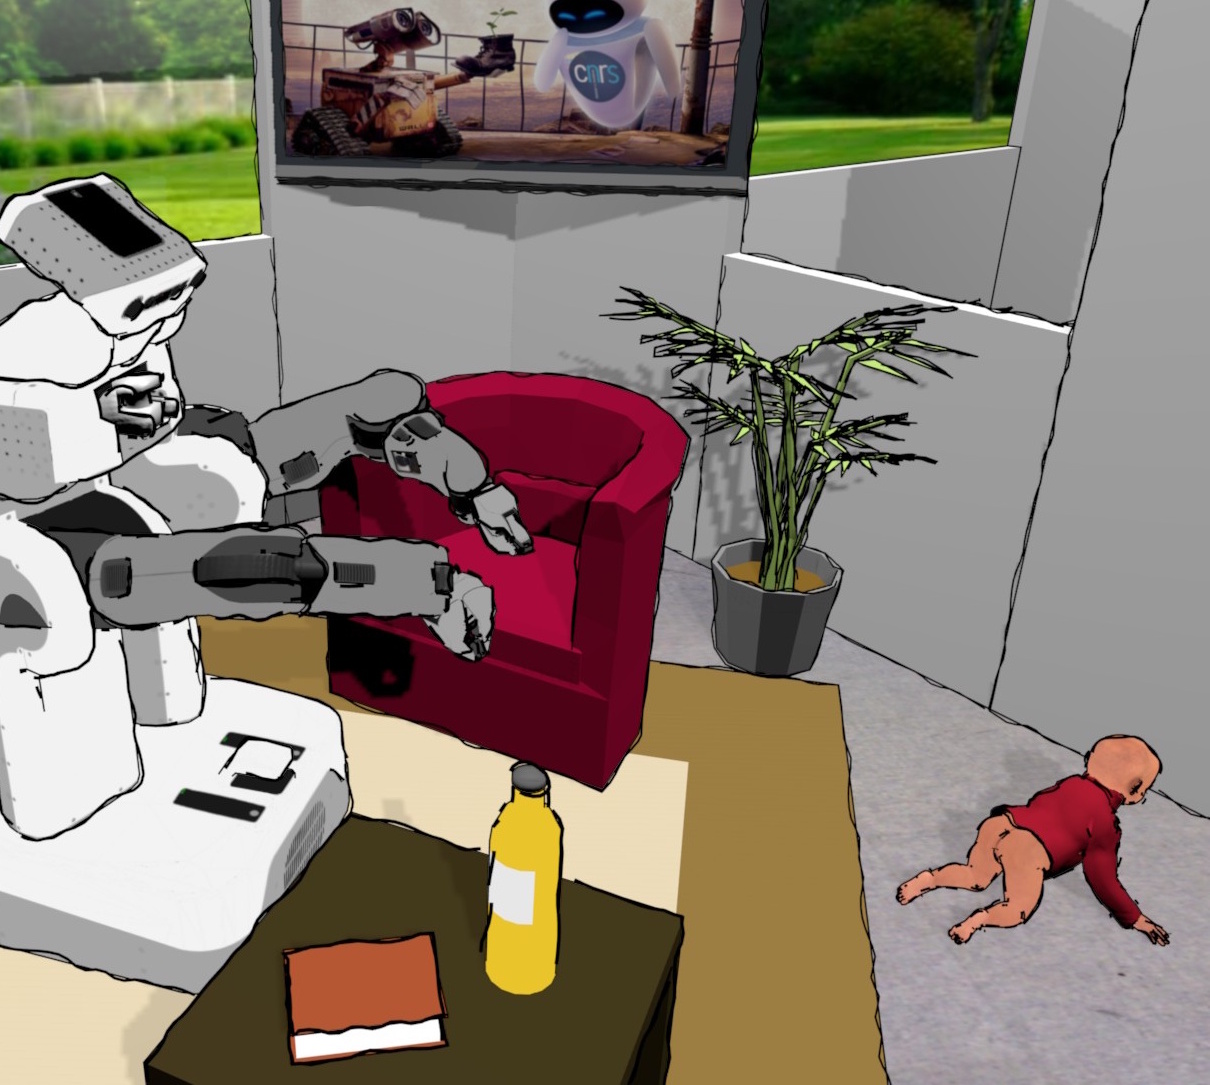
\includegraphics[width=\columnwidth]{pr2-scene.jpg}
        
        \begin{figure}

        \resizebox{\columnwidth}{!}{%
        \begin{tikzpicture}[
            yscale=1.3,
            >=latex,
            every edge/.style={<-, draw, very thick},
            every node/.style={draw, font=\sf, node distance=0.5, rounded corners,
            align=center, inner sep=5pt,fill=hriSec2Dark!50},
            classof/.style={<-, draw=black!60, dashed},
            property/.style={<-, draw=hriSec2Comp},
            propname/.style={above, draw=none, fill=none, font=\tt, inner sep=2pt},
            instance/.style={draw=hriSec1Dark, font=\sf, node distance=0.5, rounded corners,
        align=center, inner sep=5pt, fill=none}]

            \node[fill=hriSec2Comp!50] (thing) {\textbf{thing}};
            \node [fill=hriSec3CompDark!50, node distance=1.8, below left=of
            thing](sthing) {place} edge[dashed] (thing);
            \node [fill=hriSec3CompDark!50, below left=of sthing] (agent) {agent} edge (sthing);
                \node [fill=hriSec3CompDark!50, below=of sthing] (artifact) {artifact} edge (sthing);
                \node [fill=hriSec3CompDark!50, below right=of sthing] (location) {physical
                support} edge (sthing);
                \node [fill=hriSec3CompDark!50, below right=of artifact] (table) {table}
                    edge (location) edge (artifact);


            \node [node distance=1, below right=of thing] (tthing) {temporal thing} edge (thing);
                \node [below right=of tthing] (evt) {event} edge[dashed] (tthing);
                            \node [below right=of evt] (act) {action} edge (evt);

        \uncover<3->{
        \draw[dotted, thick] (-5,-3.8) -- +(13, 0);

        \node [instance, below=3 of agent] (human) {baby\_1} edge[classof, bend left] (agent);
        \node [instance, above right=of human, anchor=south] (robot) {pr2\_robot} edge[classof, bend left] (agent);
        \node [instance, right=of human, anchor=north west] (book) {book\_game\_thrones}
        edge[classof] (artifact);
        \node [instance, right=2 of robot] (ikea) {ikea\_table} edge[classof, bend
        right] (table);
        \node [instance, right=2 of book] (brown) {brown} edge[property] node[propname] {hasColor} (book);


        %}
        %\uncover<3>{
        \draw[dotted, thick] (-5,-6.2) -- +(13, 0);

        \node [instance, below=5 of act] (moving) {move\_act\_42} edge[classof] (act);
        \path (moving.west) edge [property, out=180, in=-80, looseness=1] node[propname,below] {currentlyPerforms} (human.230);

        \path (human.280) edge [property, out=-80, in=-90, looseness=3.5] node[propname,right] {looksAt} (robot.south);
        \path (ikea.south) edge [property, out=-90, in=-80, looseness=3] node[propname, auto] {isOn} (book.320);
        }
        \end{tikzpicture}
        }

        \end{figure}

    \end{multicols}

    \end{center}
\end{frame}

\imageframe{humans-pt}

{
\paper{Ros et al., {\Medium Which One? Grounding the Referent Based on Efficient HRI}, ROMAN 2010}
\begin{frame}{One Model per Agent}
        \begin{multicols}{2}
            \begin{figure}
                \resizebox{0.35\textwidth}{!}{\usebox{\ontoinstance}}
            \end{figure}
            \begin{figure}
                \resizebox{0.35\textwidth}{!}{\usebox{\ontoinstance}}
            \end{figure}
            \begin{figure}
                \resizebox{0.35\textwidth}{!}{\usebox{\ontoinstance}}
            \end{figure}
            {\vspace*{1.5cm}\hspace*{2.5cm}\huge...}
        \end{multicols}
\end{frame}
}


\maketitle

%{
%\fullbackground{background.pdf}
%\begin{frame}[plain]
%    Thank you!\\
%    \scriptsize
%    {\tt severin.lemaignan@epfl.ch}
%    \vfill
%
%\end{frame}
%}

\end{document}






